\chapter{The Speed of Light}

%\section{Pre-lab Calculations}

%\noindent
%1) What is the definition of the meter ? What is the exact value of the speed of light in vacuum?\\
%The meter  is the length of the path travelled by light in vacuum during a time interval of 1/299792458 second. The exact value for the speed of light in vacuum is 299,792,458 metres per second.

%\noindent
%2) How long does it take a light to travel a length of 1m? Using the
%time you just calculated and assuming that the uncertainty in the
%length measurement is $1~\rm cm$, calculate the uncertainty in the
%speed of light you would obtain if you were to use this measurement.
%Using again the time you just calculated and assuming that the
%uncertainty in time measurement is $0.2~\rm ns$, calculate the
%uncertainty in the speed of light you would obtain if you were to use
%this measurement. Which uncertainty is larger? \\


%\noindent
%3) Light is slowed down in transparent media such as air, water and
%glass.  The ratio by which it is slowed is called the refractive index
%of the medium. Calculate this speed of light in air if the index of
%refraction is 1.0003. Calculate (in \%) how far off is speed of light
%in the air from the speed of light in vacuum? Assuming that in our
%setup we are aiming at few $\%$ accuracy is this correction relevant
%for us?\\

\section{Safety}
The laser used in this lab is of low power.  Even so, avoid pointing the laser directly into anyone's eye.

\section{Introduction}

In this lab, you will measure the speed of light in air by measuring
the time between sending and receiving a flash of light over a known
distance.  This lab includes both logbook and Jupyter notebook
entries.

The light signal for this measurement is provided by a laser diode.
Like an LED, the photons in the laser diode are the result of
electrons and holes recombining.  The laser diode produces simulated
emission of photons from population inversion of holes and electrons
injected from p-type and n-type semiconductors into an intermediate
layer of un-doped intrinsic semiconductor.

\begin{figure}[htbp]
\begin{center}
\begin{tabular}{cc}
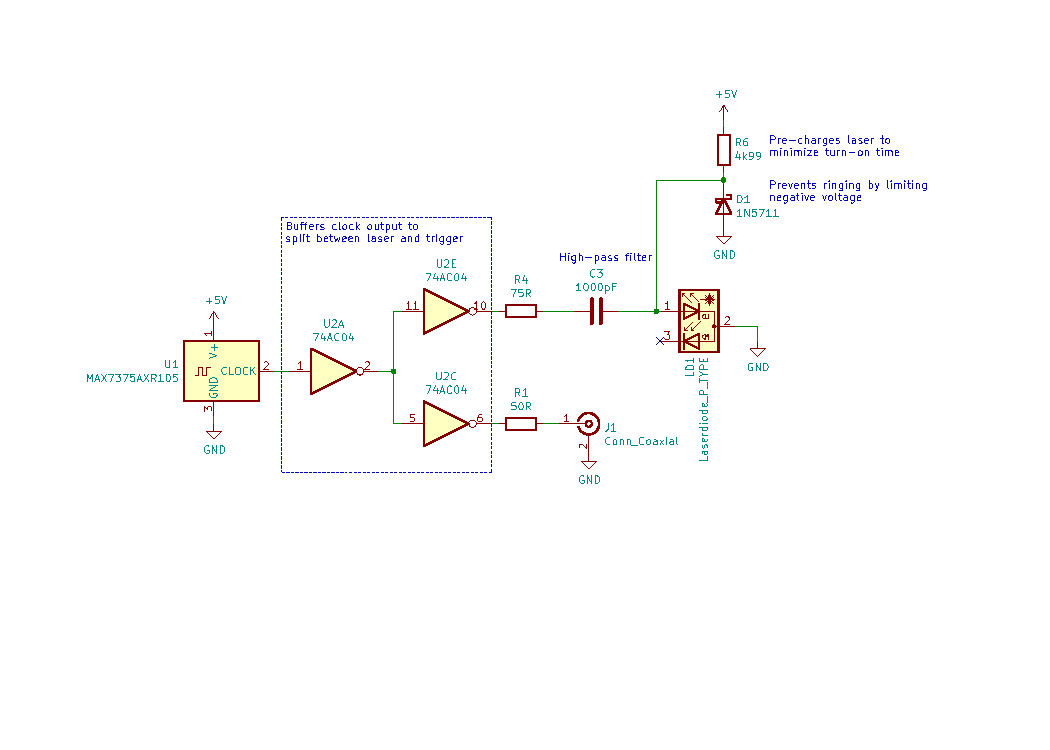
\includegraphics[width=0.9\textwidth]{figs/labs/c_air/cair_diodedriver}
\end{tabular}
\end{center}
\caption{\label{fig:clasercirc} Circuit diagram for the pulsed laser diode.}
\end{figure}

If laser light is produced continuously, we'll have no way to measure
a time difference between sending and receiving the pulse.  Instead,
we'll produce a brief pulse of laser light and a reference signal to
indicate the time at which the pulse was sent.  The circuit for pulsed
laser diode assembly we will be using is shown in
Fig.~\ref{fig:clasercirc}.  You will recognize the passive components
consisting of resistors, diodes, and capacitors.  The MAX7375 (square
symbol) is a silicon oscillator which produces a $1~\rm MHz$ square
wave function.  The 74C04 (triangle symbol) is technically an
inverter, but here they are used to simply produce two independent
copies of the square wave function output.  One copy of the square
wave function is sent to a BNC connector, as the time reference for
sending the laser pulse.  The other copy is send through a capacitor,
which acts as a high-pass filter, converting the step function into
very narrow positive and negative pulses.  The diode D1 rectifies this
AC signal, so that only the positive signal is used to drive the laser
diode, causing a brief pulse of laser light, in sync with the square
wave signal which will be available on the scope.

\begin{figure}[htbp]
\begin{center}
\begin{tabular}{cc}
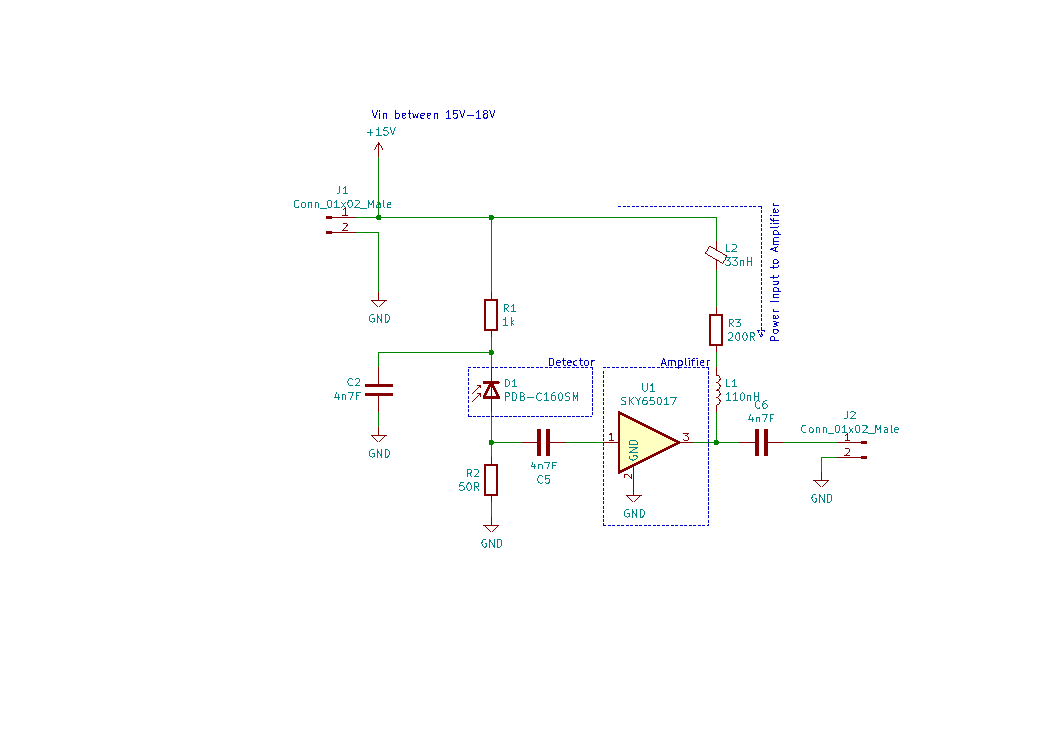
\includegraphics[width=0.7\textwidth]{figs/labs/c_air/cair_detector}
\end{tabular}
\end{center}
\caption{\label{fig:cdetectorcirc} Circuit diagram for photodiode detector.}
\end{figure}

We'll detect the flash of light using a photo-diode.  The photo-diode
is placed in reverse bias, creating a depletion zone.  When photons
strike the depletion zone, they excite electrons to create
electron-hole pairs, which allows a current to flow.  The receiver
circuit is shown in Fig.~\ref{fig:cdetectorcirc}.  The photo-diode D1
is held under reverse bias by the externally supplied DC voltage.  The
current pulse created when the laser light reaches the photo-diode is
amplified by the SKYC5017 broadband amplifier.  All amplifiers have
limits to their bandwidth, but this amplifier is fast enough to handle
the brief laser pulse that we are sending.  The input connector for
this device has an internally generated DC voltage, so we use the
capacitor C5 to isolate this DC voltage from our circuit.  The
high-frequency AC signal pulse we wish to amplify will see this
capacitor as effectively a short-circuit.  All amplifiers require
external DC power, but this one is a bit peculiar in that the DC power
is supplied at the output pin.  This explains the use of inductors L1
and L2 and capacitor C6.  Remember inductors are a short-circuit to DC
and an open circuit to AC, where as capacitors are an open-circuit to
DC and a short-circuit to AC.  The DC supply is provided to the output
pin through the inductors, but the amplified AC output signal passes
through the capacitor.


\section{Experimental Setup}

\begin{figure}[htbp]
\begin{center}
\begin{tikzpicture}%[show background grid] %% Use grid for positioning, then turn off
    \node[anchor=south west,inner sep=0] (image) at (0,0,0) {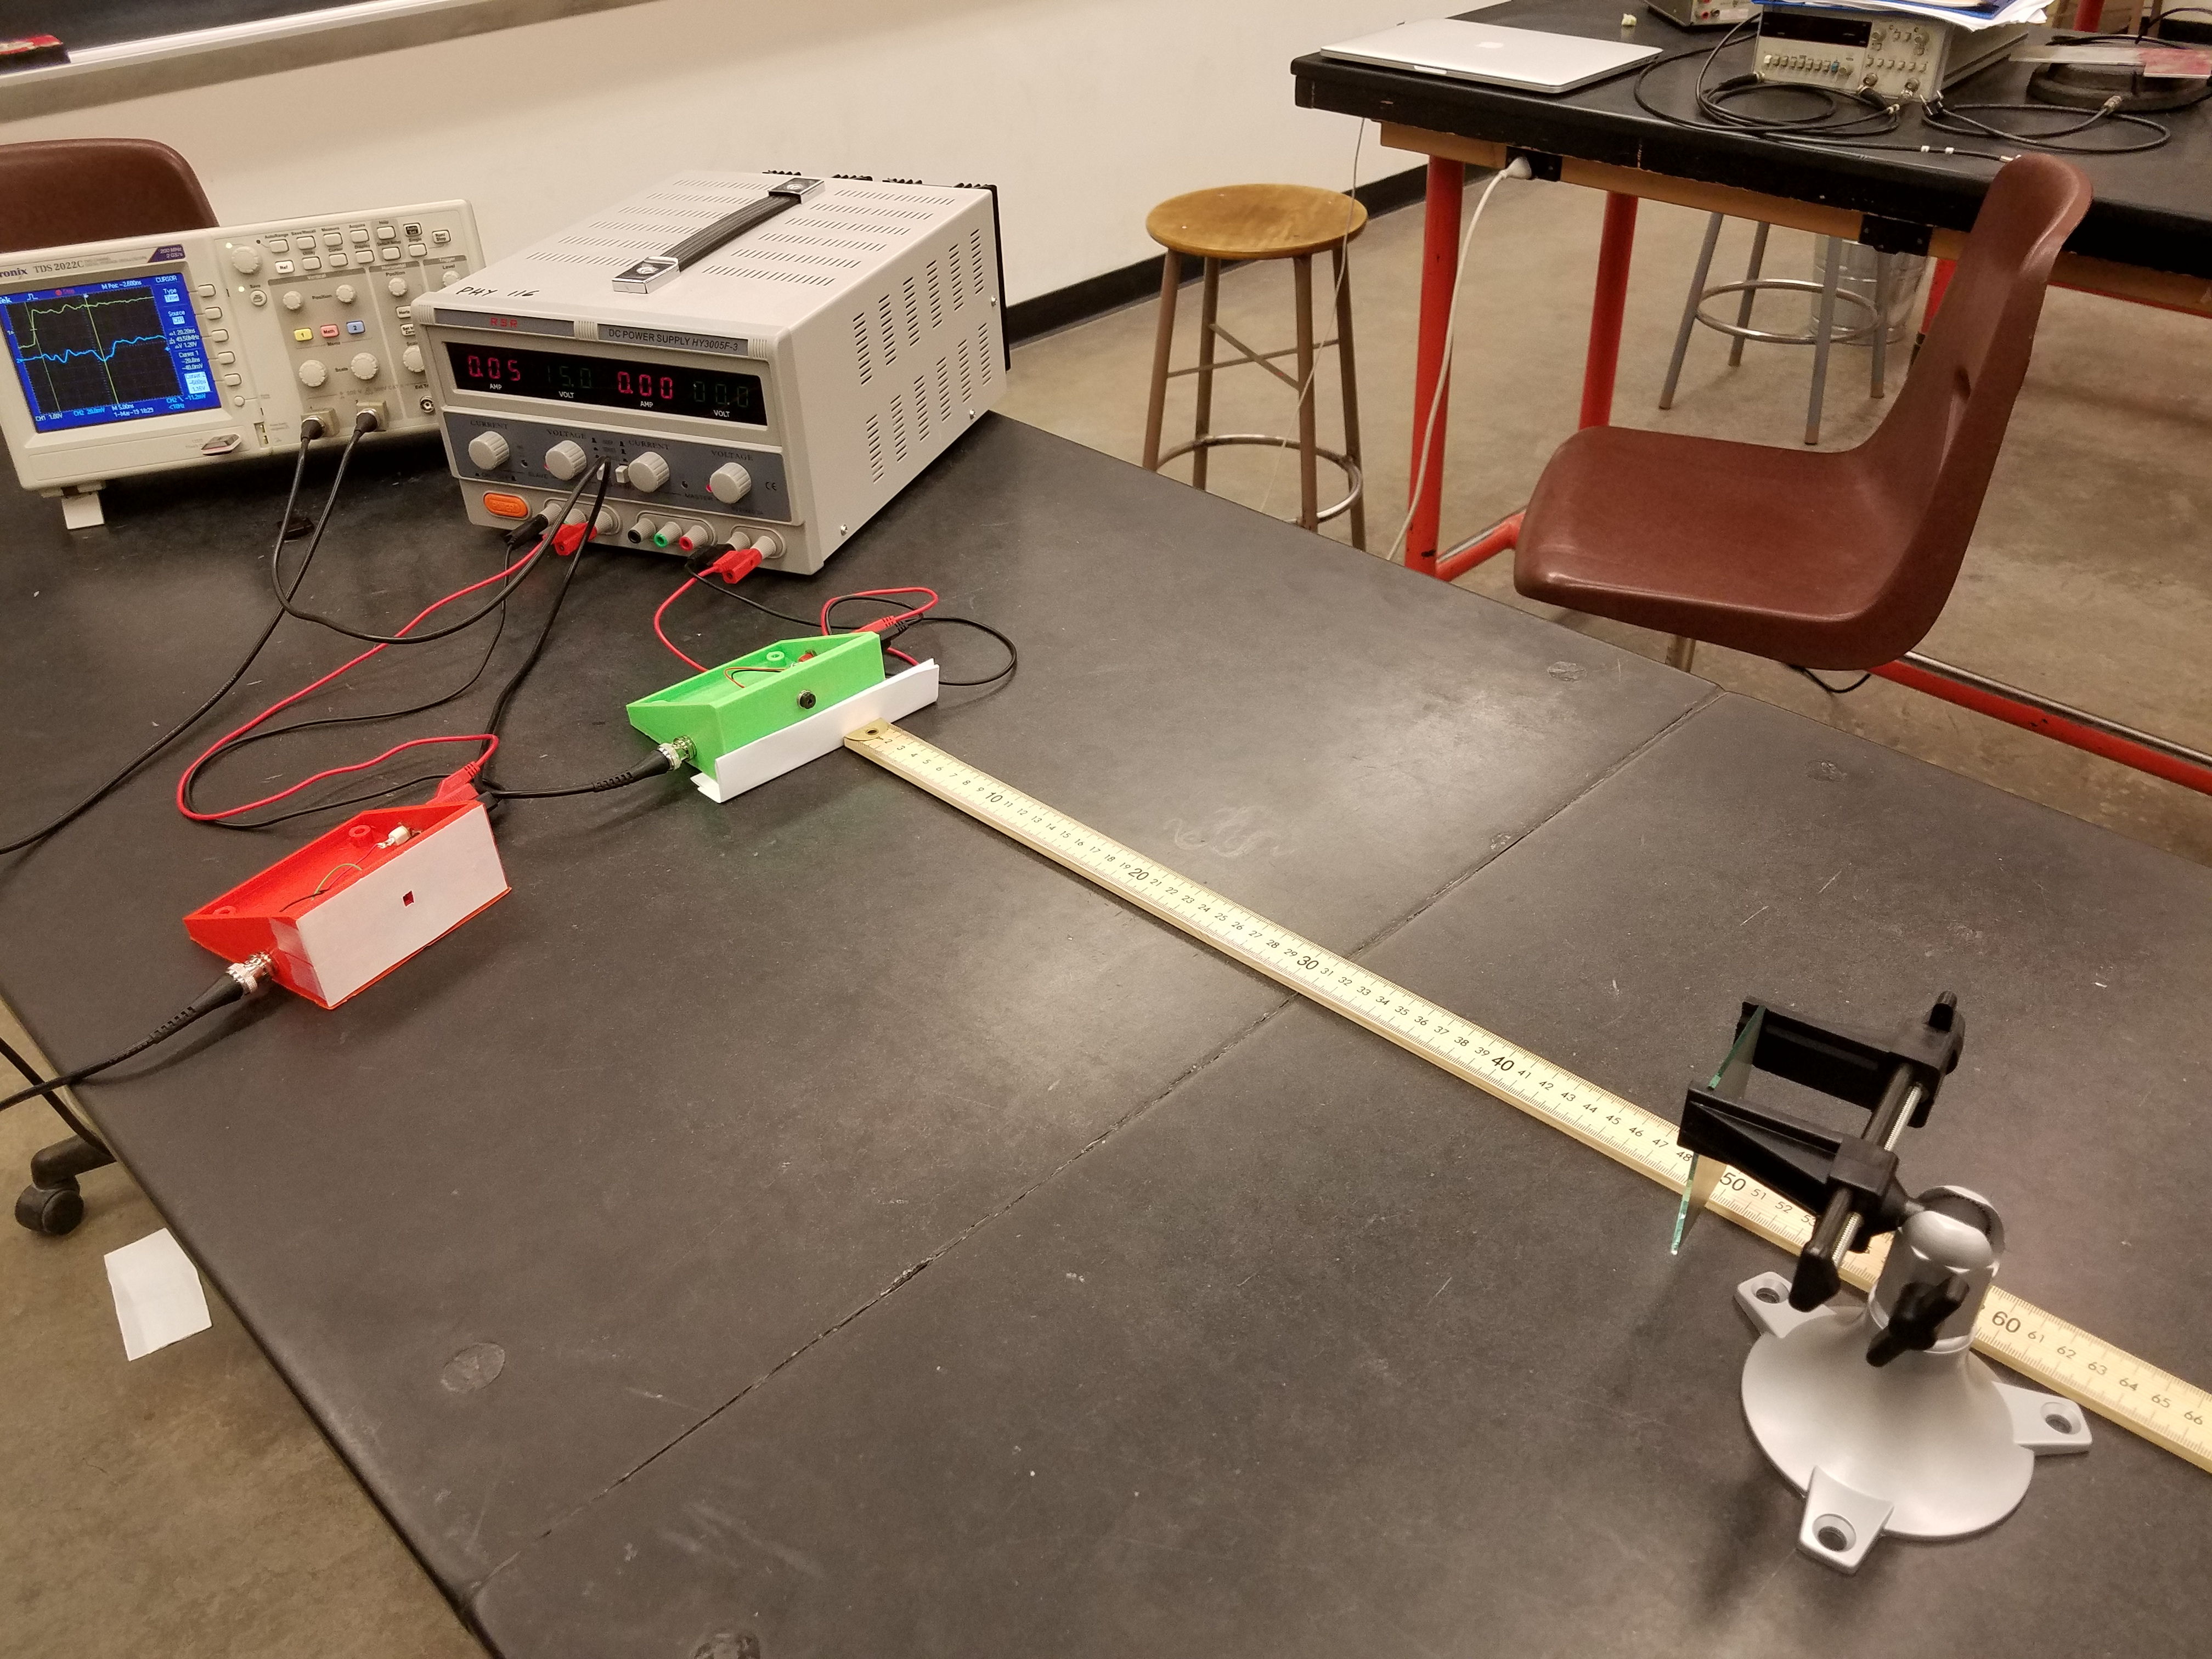
\includegraphics[width=0.7\textwidth]{figs/labs/c_air/setup.jpg}};
    %\node[right](X) at (10.0,5.1) {\parbox{3cm}{\flushleft Trigger (yellow)}};
    \draw [dashed,red,thick] (4.55,5.4) -- (9.5,2.75);
    \draw [dashed,red,thick] (2.35,4.3) -- (9.5,2.75);
\end{tikzpicture}
\end{center}
\caption{\label{fig:csetup} Setup.}
\end{figure}

The setup is shown in Fig.~\ref{fig:csetup}.  You will use your
bench-top DC power supply to power the pulsed laser diode and the
photo-diode receiver assemblies.  The right most pair of output from
your supply provides a fixed $5~\rm V$ DC output, which you will use
to power the pulsed laser diode assembly (transmitter).  The
transmitter is housed in the green box. The reference signal for the
transmitter is output on the BNC connector, and should be connected to
your channel 1 of your scope, {\bf using a $50~\rm \Omega$ terminator.}

The photo-diode receiver circuit is housed in the red box.  It should
be powered at $10~\rm V$ from your bench-top DC power supply.  The
amplified signal output on the BNC connector should be connected to
channel 2 of your scope, {\bf using a $50~\rm \Omega$ terminator.}

%To suppress high-frequency noise, you can try installing RF chokes
%around your coaxial cable near the receiver and transmitter.  

\begin{figure}[htbp]
\begin{center}
\begin{tabular}{cc}
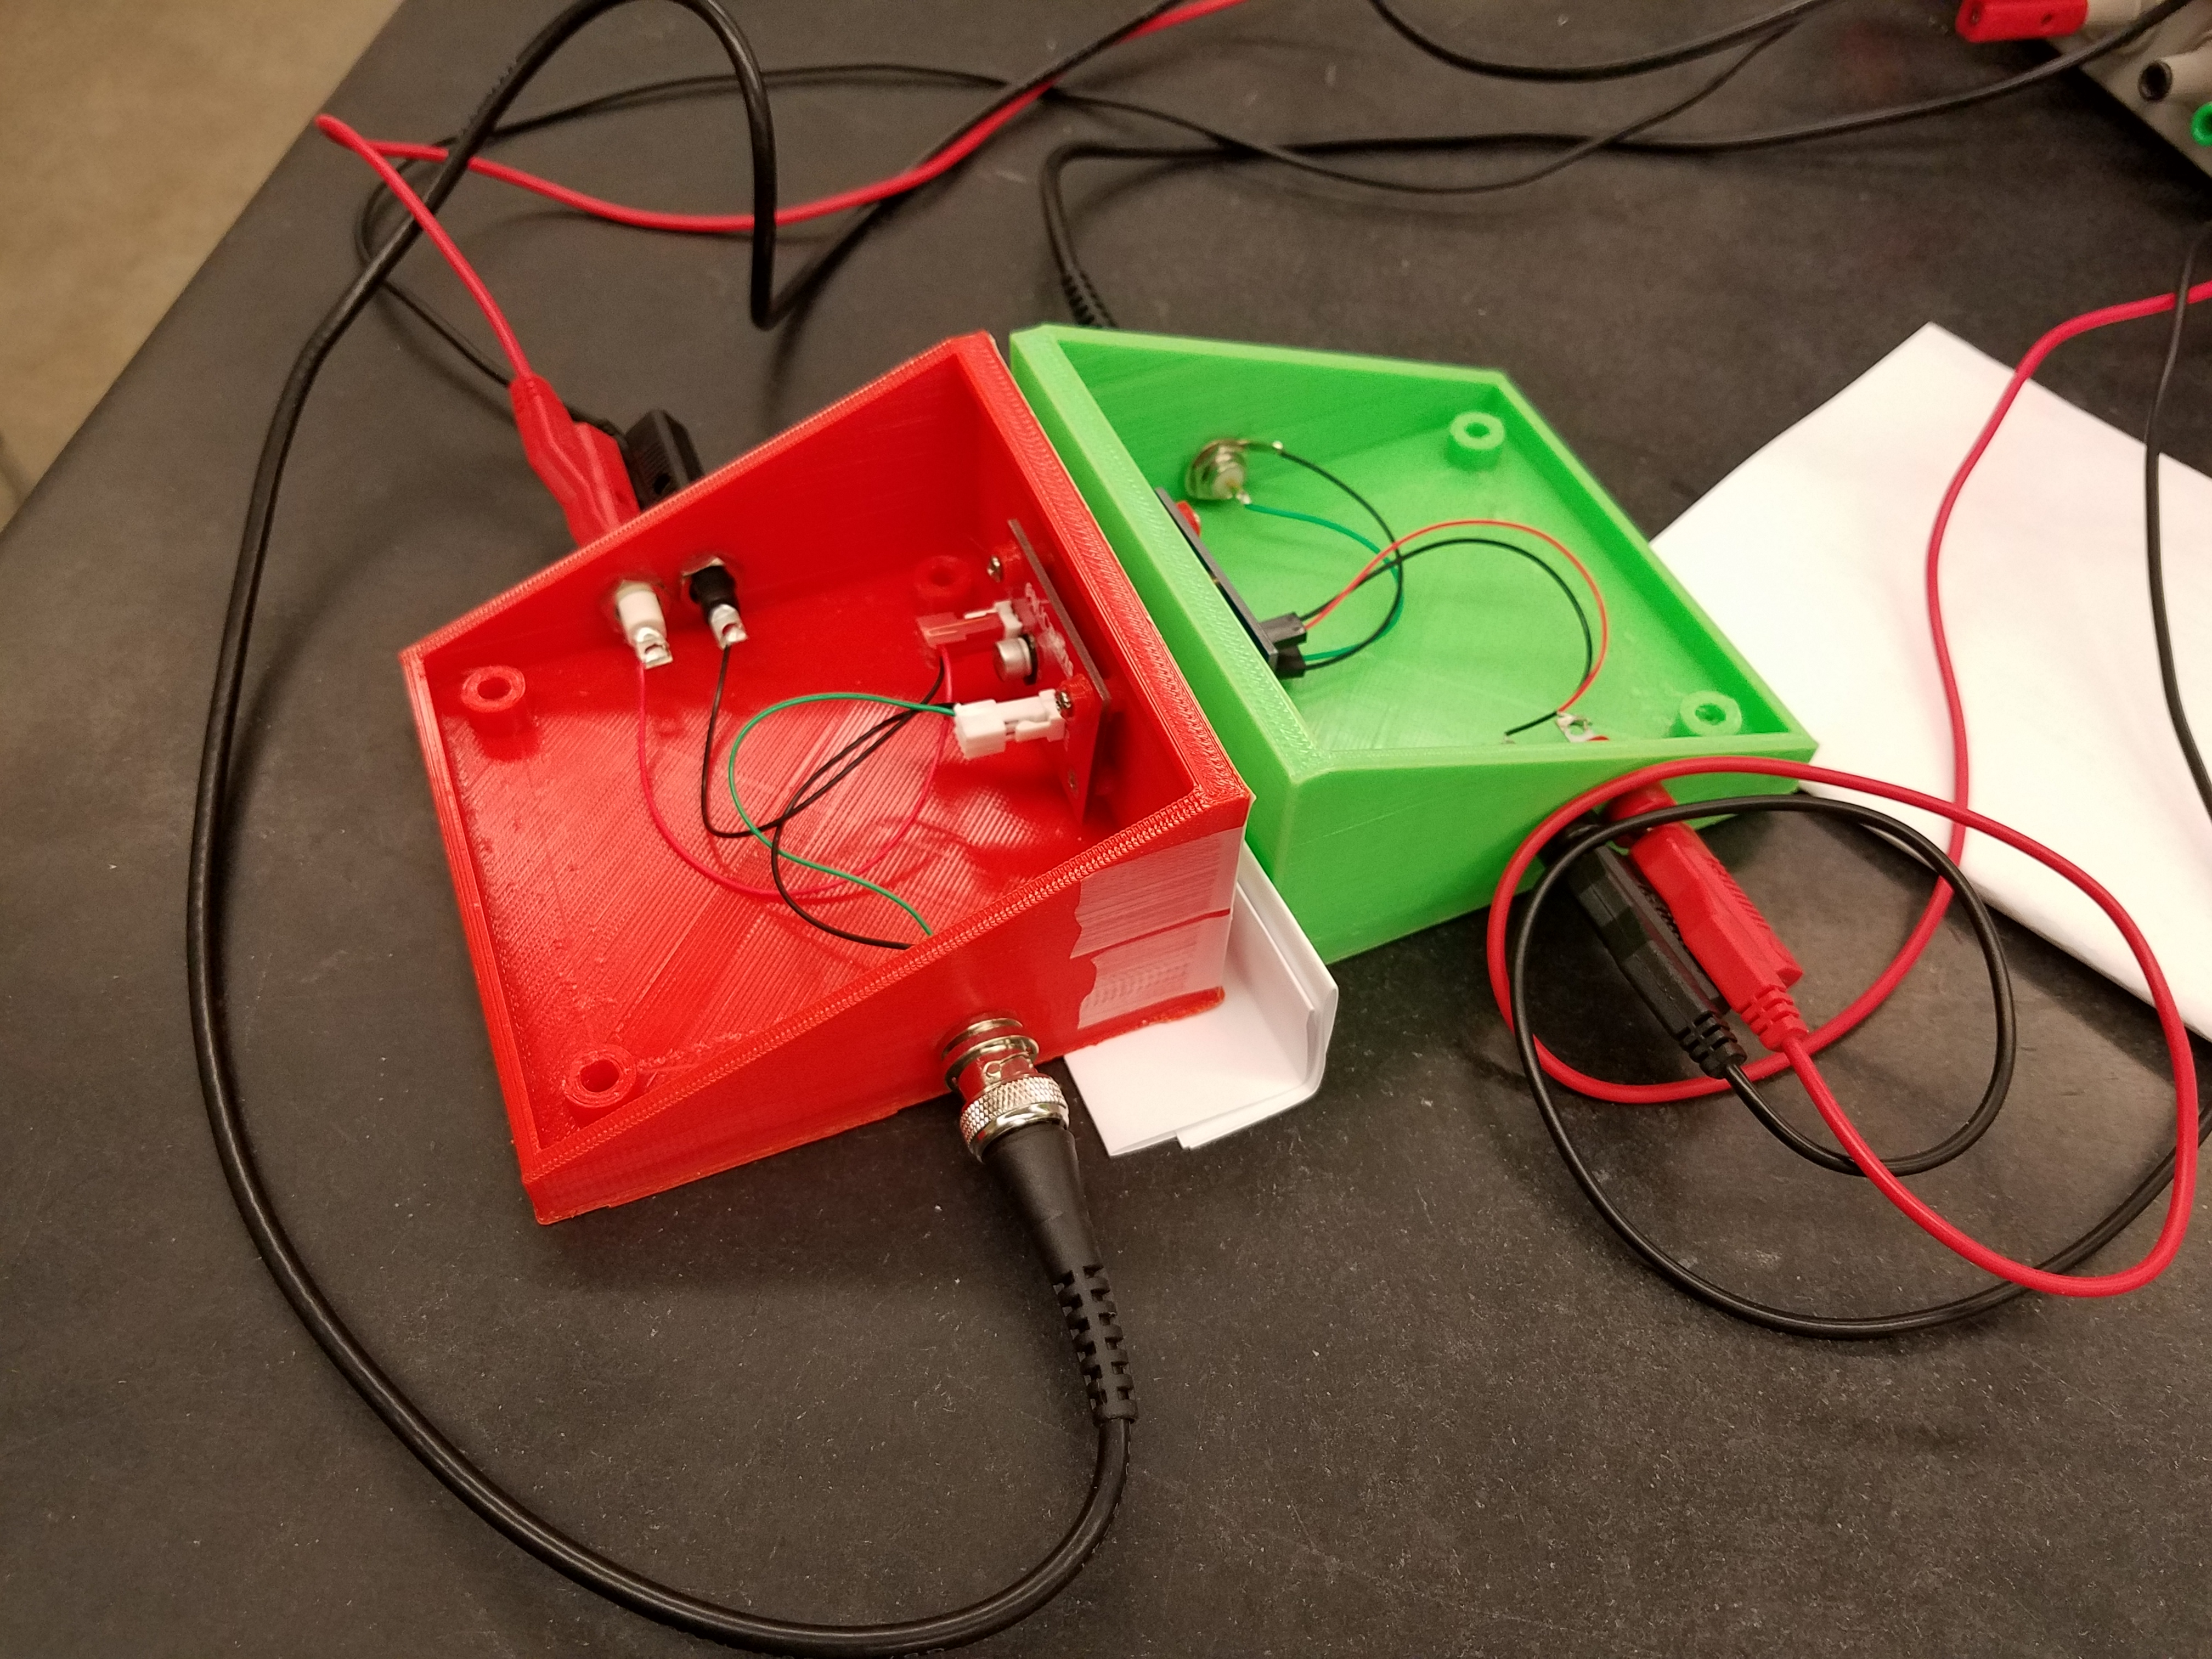
\includegraphics[width=0.7\textwidth]{figs/labs/c_air/tzero.jpg}
\end{tabular}
\end{center}
\caption{\label{fig:ctzero} Initially, point the laser directly into the receiver.}
\end{figure}

\begin{figure}[htbp]
\begin{center}
\begin{tabular}{cc}
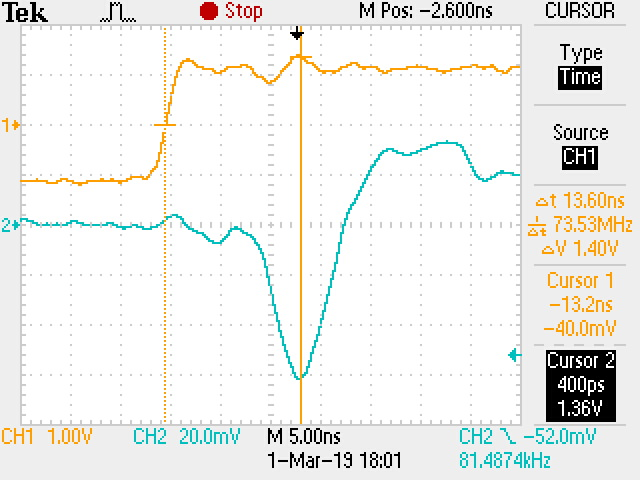
\includegraphics[width=0.7\textwidth]{figs/labs/c_air/time_peak.jpg}
\end{tabular}
\end{center}
\caption{\label{fig:ctime} Measure the time interval from the receiver reference signal (yellow, offset by two divisions) crosses zero to the lowest point in the signal pulse (blue).}
\end{figure}

To test your setup and the equipment, point the laser directly into
the receiver as shown in Fig.~\ref{fig:ctzero}.  Use folded printer
paper to adjust the height and orientation of the boxes as needed.  

Make certain that your digital oscilloscope has a bandwidth of 100
MHz.  The receiver signal is the most intermittent, so to avoid seeing
empty wave-forms, you should always trigger on the receiver signal.
Set both channels to AC coupling and make certain that the bandwidth
limit is off.  Set the time-scale to 5 nanoseconds.


An example of the timing measurements you will be making is shown in
Fig.~\ref{fig:ctime}.  Ideally, when making a timing measurement, you
should use a sharp edge.  This is why the reference signal is measured
on the rising edge.  The receiver signal, however, is quite noisy, so
the edge is easily distorted.  A slightly more reliable measurement
comes from the using the minimum of the pulse.  There is significant
variation of the pulse height, so it helps to set the trigger level to
only select the largest pulses (by moving the trigger threshold as far
toward the bottom of the screen as possible).  Because of timing
jitter, you will acquire a single waveform to make each time
measurement, using the scopes run/stop or the single button.

\begin{measurement}
Measure the time offset ($\Delta t$ at zero distance).  Each student
should make at least three measurements, from three different
waveforms.  Despite the jitter, you should see that the time interval
measurements are fairly stable, varying by about 0.2 nanoseconds, the
cursor resolution at the five nanosecond scale.
\end{measurement}

\section{Speed of Light Measurement}

\begin{figure}[htbp]
\begin{center}
\begin{tabular}{cc}
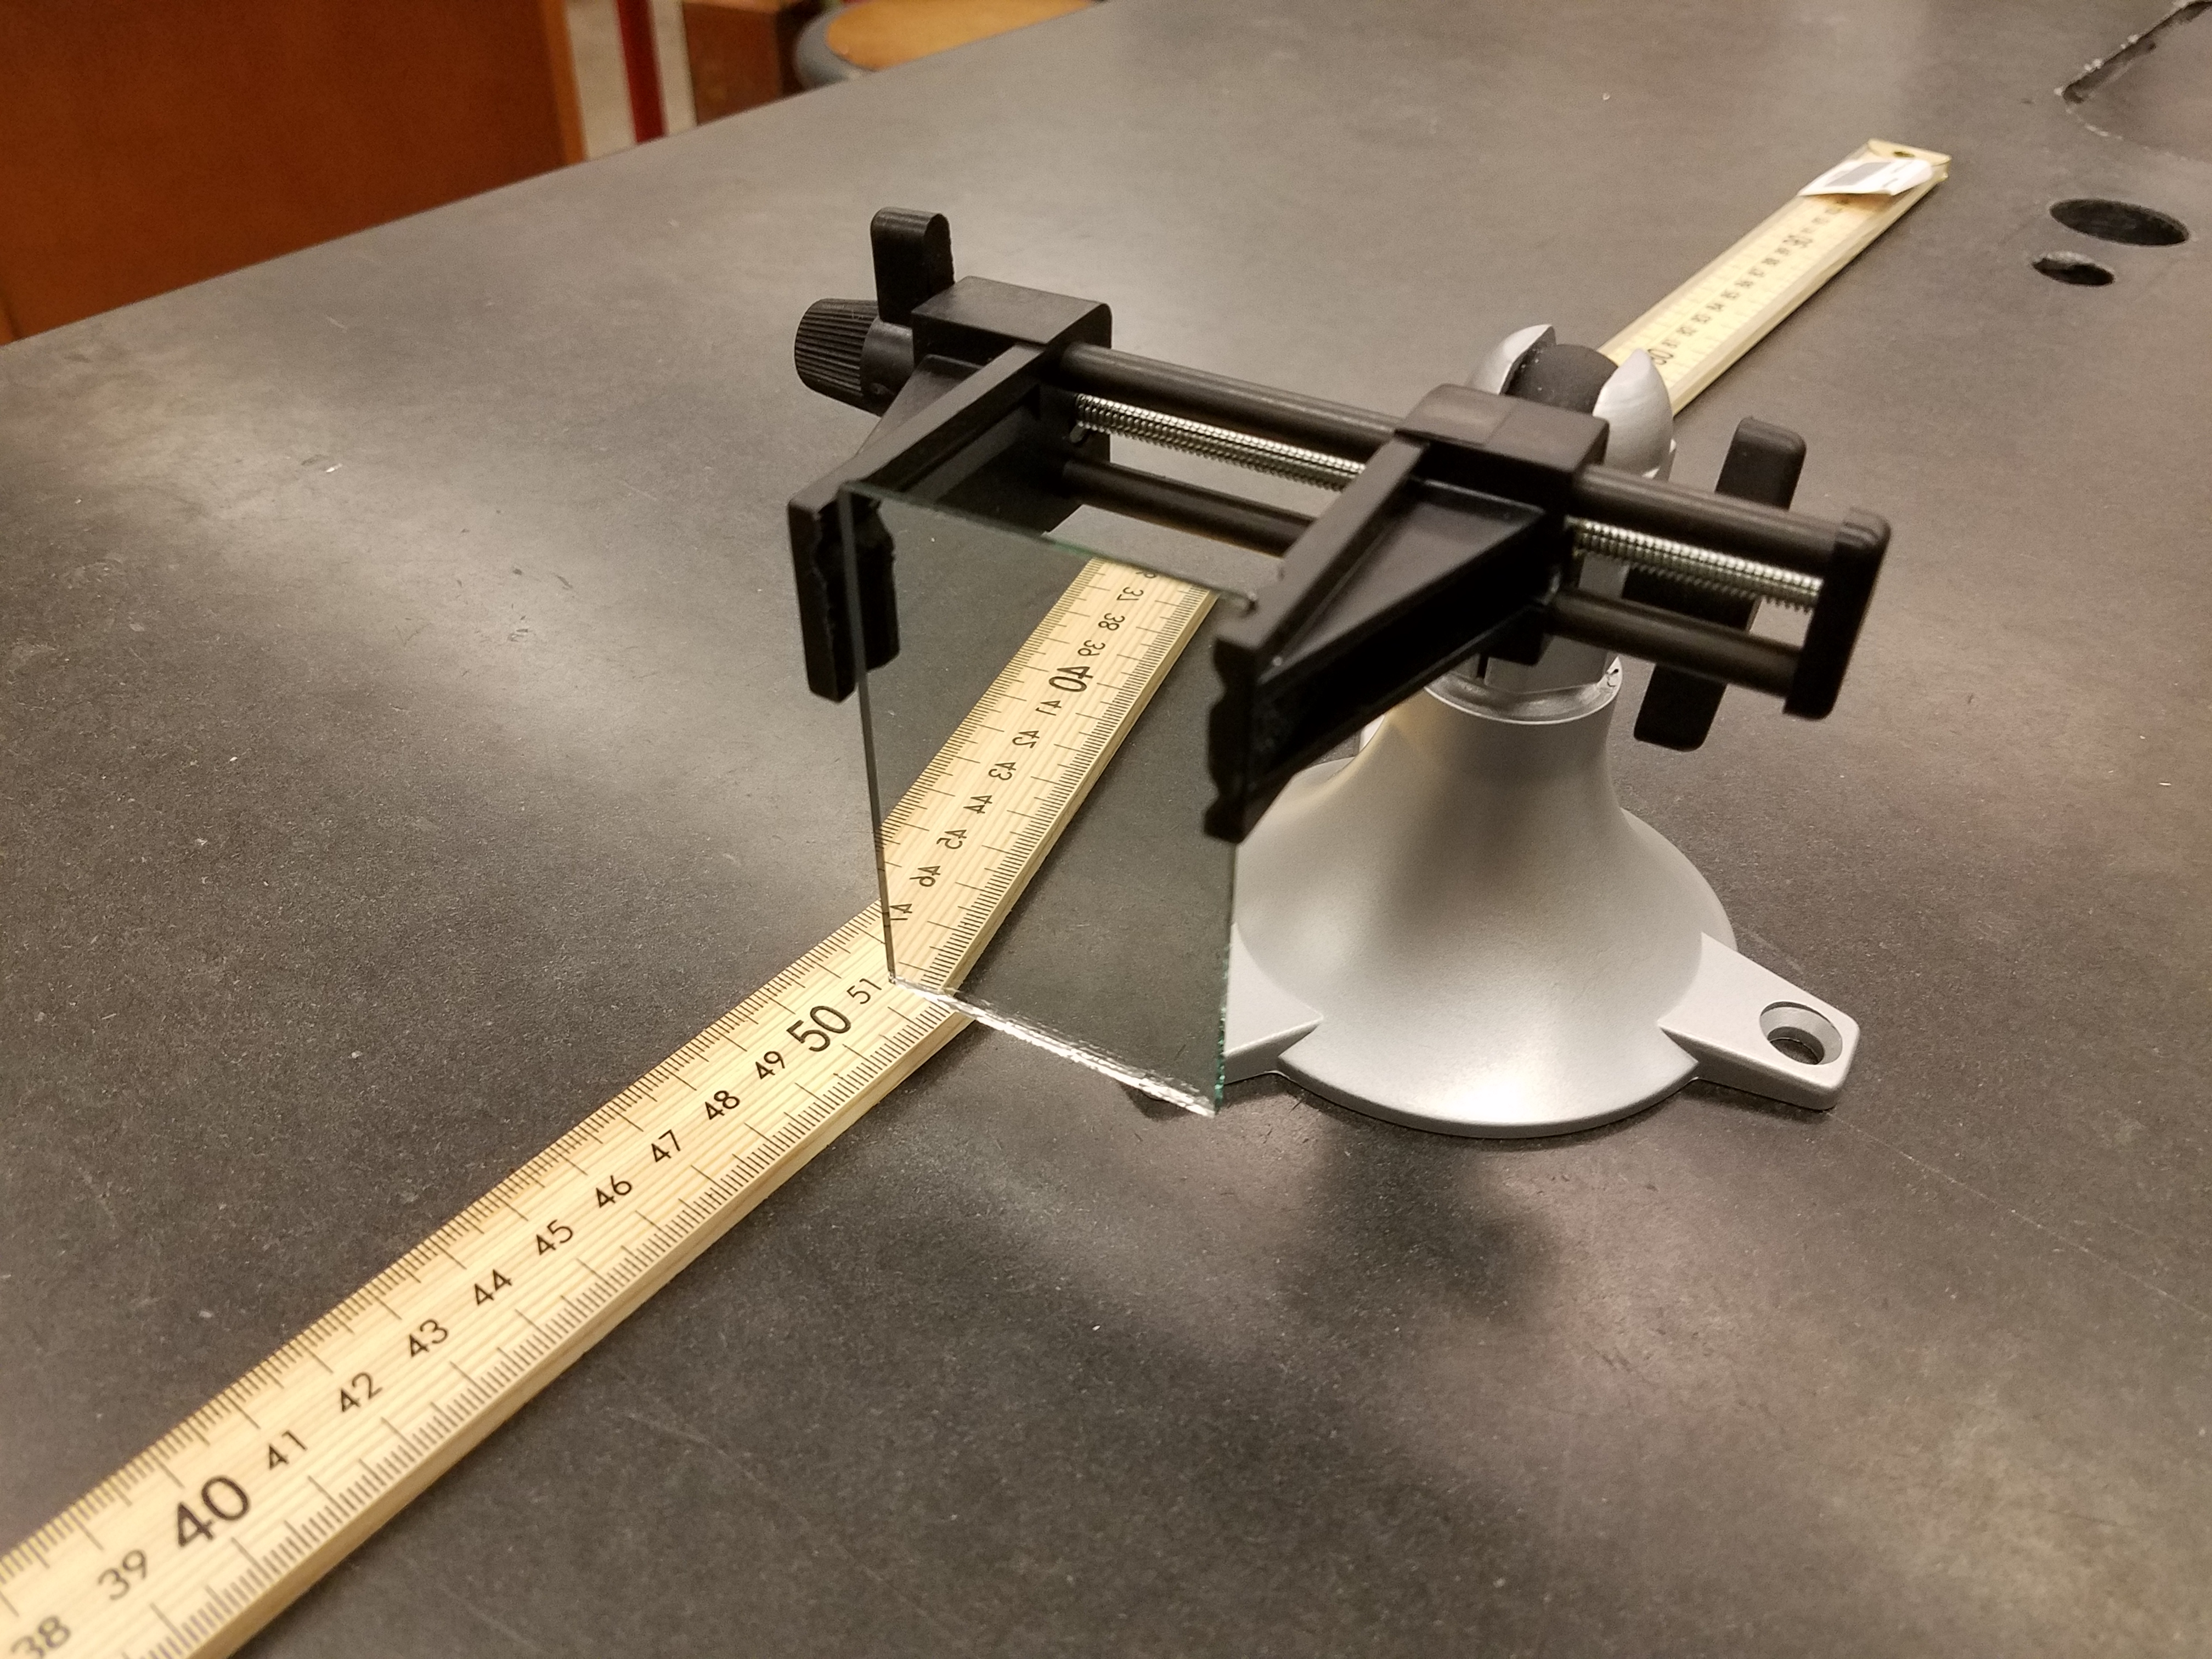
\includegraphics[width=0.7\textwidth]{figs/labs/c_air/mirror.jpg}
\end{tabular}
\end{center}
\caption{\label{fig:mirror} Mirror held in a swivel-mount vise}
\end{figure}

Install a mirror in your swivel mount vise as shown in
Fig.~\ref{fig:mirror} Move the transmitter to point the beam down the
long access of your lab bench.  Place the mirror approximately 25 cm
away from the transmitter as measured with a meter stick.  Using a
piece of white paper to track the beam spot, adjust the transmitter
until the beam is pointed at the mirror.  Place the receiver next to
the transmitter and pointed at the mirror.  Adjust the mirror until
the beam is directed back to the receiver. 

Once you have the beam pointed toward the receiver, orient your scope
display so that you can see it clearly from the mirror.  Set the
trigger to just below the noise level, and adjust the mirror until the
beam points into the receiver and a clear signal appears on your
scope.  Tighten the swivel mount to hold the mirror in place.  You may
find that the mirror moves slightly after you remove your hands and
the signal is lost.  If this is happening, try gradually tightening
and adjusting the mirror, or lightly tapping it while the swivel-mount
is tight.  Continue adjusting until you have a clear signal.  

\begin{measurement}
Each lab partner should make their own measurement of
the time difference between the transmitter and receiver signals, and
record all measurements in your logbooks.  Then each lab partner
should make a measurement of the total beam distance to the nearest
0.5 cm.  Record all measurements in your logbooks.  Estimate the
uncertainty on your measurement.  The resolution of the cursor time
measurement at the 5 ns scale is 0.2 ns.  The meter stick has a
resolution of about 0.5 cm.  If your measurements are consistent with
one another, you can use these resolutions as your uncertainties.
From these measurements and the timing offset measured previously,
calculate the speed of light and an uncertainty.
\end{measurement}

\begin{measurement}
Repeat the procedure for previous measurement (at about 25 cm) for a starting position of the
mirror at 50 cm, 75 cm, and 100 cm.
\end{measurement}

\section{Analysis}

\begin{plot}
Plot the data with the x-values populated by the
quantity with smaller uncertainty and y-values populated by the
quantity with the larger uncertainty. Include x and y-uncertainties in
the plot. Perform a straight line fit using {\tt curve{\_}fit}
function. Include y-uncertainties in the fit and be sure to set {\tt absolute{\_}sigma=True}.  From the fit values
calculate the speed of light together with its uncertainty.
\end{plot}

A major source of systematic uncertainty in this measurement comes
from the timing measurement.  The transmitter reference has a nice
sharp edge, but the signal pulse is distorted by amplification.  As
the distance traveled by the light pulse increases, the signal becomes
smaller, and the signal shape changes, which changes the measured time
interval.  This introduces a non-linearity into the relationship between
the distance and your measured time.

\begin{plot}
To estimate the size of this effect, repeat the analysis but with \\ {\tt
  absolute{\_}sigma=False}.  This setting instructs the {\rm
  curve{\_}fit} function to adjust the uncertainties until they are
consistent with the linear relationship assumed in the fit.  You can
then interpret the parameter uncertainty as including both the
statistical uncertainty and the systematic uncertainty due to this
non-linearity.
\end{plot}

